\documentclass[11pt]{extarticle}
\usepackage[margin=1.27cm]{geometry}
\usepackage{setspace}
\usepackage{fontspec}
% \usepackage[T1]{fontenc}
% \usepackage[utf8]{inputenc}
\usepackage{amsmath,txfonts,amssymb,nicefrac,mathtools,pifont} %for math
\usepackage{array,tabularx,multirow,fmtcount} %for tables
\usepackage{tikz, pgfplots} %for diagram
\usepackage{multicol} %for multiple column
\usepackage{enumerate,enumitem,adjustbox} %for ordered list
\usepackage{graphicx,subcaption,wrapfig,tcolorbox} %for figure
\usepackage{xparse} %for commands & environments
\usepackage{lipsum} %miscellaneous
\usepackage{colortbl,xcolor,soul} %for default table & border

% #ANCHOR Font settings
\setmainfont{Oxygen}
\newfontfamily\banglafont[Script=Bengali]{Baloo Da 2}
\newfontfamily{\lstsansserif}{IBM Plex Mono}
\renewcommand{\normalsize}{\fontsize{11.5pt}{13pt}\selectfont}


\setlength{\arrayrulewidth}{0.35 pt}
\definecolor{border}{HTML}{A1A1AA}
\arrayrulecolor{border}


% #ANCHOR Document settings
\linespread{1.45}
\setlength\parindent{0pt}
\setlength\parskip{16pt}
\setlist[enumerate]{noitemsep}
\usetikzlibrary{shapes.geometric,decorations.pathreplacing,trees,arrows,positioning,shapes,fit,calc,decorations.markings, decorations.text}
\tikzset{every node/.append style={font=\footnotesize}}
\usepgfplotslibrary{fillbetween}
\pgfdeclarelayer{background}
\pgfsetlayers{background,main}
\pgfplotsset{compat=1.18}
\columnseprule=1pt
\everymath{\displaystyle}
% #ANCHOR Hypernation
\tolerance=1
\emergencystretch=\maxdimen
\hyphenpenalty=10000
\hbadness=10000
\newlength{\colWidth}



% #ANCHOR Colors
\definecolor{azure(colorwheel)}{rgb}{0.0, 0.5, 1.0}
\definecolor{carminepink}{rgb}{0.92, 0.3, 0.26}
\definecolor{orange}{rgb}{0.9, 0.55, 0.22}
\definecolor{violet}{rgb}{0.60, 0.45, 1}
% Syantax Highlighting Colors
\definecolor{keyword}{HTML}{D73A4A}
\definecolor{number}{HTML}{015CC5}
\definecolor{comment}{HTML}{6A737D}
\definecolor{string}{HTML}{1D825E}
\definecolor{function}{HTML}{743FD1}
\definecolor{orange}{HTML}{CF7842}
\definecolor{codeblack}{HTML}{24292F}
\definecolor{divider}{HTML}{A1A1AA}
\definecolor{border}{HTML}{D1D1D1}


% #ANCHOR Ordered & Unordered List
\setlist[itemize,1]{left=0cm, label={\textbullet}}
\setlist[itemize,2,3,4,5,6,7,8,9,10]{left=0.6cm, label={\textbullet}}
\setlist[enumerate,1]{left=0cm}
\setlist[enumerate,2,3,4,5,6,7,8,9,10]{left=0.6cm}
\setul{0.5ex}{0.125ex}



% #ANCHOR Colored Box
\let\oldul\ul
\renewcommand{\ul}[2][keyword]{\text{\setulcolor{#1}\oldul{#2}}}
\newcommand{\redbox}[1]{%
{\color{red}\fbox{\color{black}#1}}
}
\newcommand{\red}[1]{%
\textcolor{red}{#1}
}
\newcommand{\redeq}[1]{%
\text{\color{red}$#1$}
}
\newcommand{\mred}[1]{%
\textcolor{keyword}{#1}
}
\newcommand{\mredeq}[1]{%
\textcolor{keyword}{$#1$}
}
\newcommand{\blue}[1]{%
% {\color{number}#1\hspace{-0.4ex}}
\textcolor{number}{#1}
}
\newcommand{\blueeq}[1]{%
\text{\color{number}$#1$}
}
\newcommand{\cyanbox}[1]{%
{\color{teal}\fbox{\textcolor{black}{#1}}}
}
\newcommand{\cyan}[1]{%
\textcolor{teal}{#1}
}
\newcommand{\pink}[1]{%
\textcolor{magenta}{#1}
}
\newcommand{\orange}[1]{%
\textcolor{orange}{#1}
}
\newcommand{\violet}[1]{%
{\color{violet}#1}
}
\newcommand{\cyaneq}[1]{%
\text{\color{teal}$#1$}
}
\newcommand{\gray}[1]{%
\textcolor{comment}{#1}
}
\newcommand{\pinkeq}[1]{%
\text{\color{magenta}$#1$}
}
\renewcommand{\columnseprulecolor}{\color{divider}}




% #ANCHOR Tabular commands
\newcolumntype{P}[1]{>{\centering\arraybackslash}p{#1}}
\newcolumntype{M}[1]{>{\centering\arraybackslash}m{#1}}
\newcolumntype{C}{>{\centering\arraybackslash}X}
\newcommand{\rspan}[2]{\multirow{#1}{*}{#2}}
\newcommand{\thc}[1]{%
\multicolumn{1}{|c|}{\textbf{#1}}
}
\newcommand{\thcx}[1]{%
\multicolumn{1}{|C|}{\textbf{#1}}
}
\newcommand{\thl}[1]{%
\multicolumn{1}{|l|}{\textbf{#1}}
}
\newcommand{\thr}[1]{%
\multicolumn{1}{|r|}{\textbf{#1}}
}
% Adjusting arraystretch to modify vertical padding
\renewcommand{\arraystretch}{1.25}
% Adjusting tabcolsep to modify horizontal padding
\setlength{\tabcolsep}{10pt}



% #ANCHOR Math commands
\newcommand{\set}[1]{\{$#1$\}}
\newcommand{\tabs}{\ \ \ \ \ \ }
\newcommand{\tab}{\ \ \ }
\newcommand{\cmark}{\ding{51}}%
\newcommand{\xmark}{\ding{55}}%
\newcommand{\boldi}[1]{\boldsymbol{#1}}%
\newcommand{\wspace}{\ \ = \ \ }



% #ANCHOR New commands
\newcommand{\Title}[1]{%
   \begin{center}
      \textbf{\Large{#1}}
   \end{center}
}
\newcommand{\Heading}[1]{%
   \par\vspace{\dimexpr -\baselineskip + 16pt}
   {\fontsize{12pt}{13pt}\selectfont\textbf{#1}}
   \par\vspace{\dimexpr -\baselineskip + 6pt}
}
\newcommand{\BuleHeading}[1]{%
   \par\vspace{\dimexpr -\baselineskip + 16pt}
   {\fontsize{12pt}{13pt}\selectfont\textbf{\textcolor{number}{#1}}}
   \par\vspace{\dimexpr -\baselineskip + 6pt}
}
\newcommand{\CHeading}[1]{%
   \par\vspace{\dimexpr -\baselineskip + 16pt}
   \hspace{\fill}
   {\fontsize{12pt}{13pt}\selectfont\textbf{#1}}
   \hspace{\fill}
   \par\vspace{\dimexpr -\baselineskip + 6pt}
}
\newcommand{\Section}[1]{%
   \par\vspace{\dimexpr -\baselineskip + 16pt}
   \hspace{\fill}
   {\fontsize{13pt}{13pt}\selectfont\textbf{#1}}
   \hspace{\fill}
   \par\vspace{\dimexpr -\baselineskip + 6pt}
}
\newcommand{\seteqno}[1]{%
   \ \cdots \ \cdots \ \cdots \ (#1)
}
\newcommand{\eqor}{%
   \Rightarrow \ \ 
}
\newcommand{\tsub}[1]{%
\textsubscript{#1}\hspace{-0.45ex}
}
\newcommand{\tsup}[1]{%
\textsuperscript{#1}\hspace{-0.45ex}
}
\newcommand{\cbox}[2][cyan]{
\tikz\node[draw=#1,circle,inner sep=2pt,baseline=(a.base)](a){#2};
}
\newcommand{\hrline}{%
\vspace{1ex} {\color{gray}\hrule} \vspace{4ex}
}
\newcommand{\divideX}[1][divider]{{\hspace{1ex}\color{#1}{\vrule}\hspace{1ex}}}
\newcommand{\Reference}[2][Reference]{

\vspace{-0.5\baselineskip}
\begin{center}
   {\fontspec{Merriweather}\textbf{#1:} \textit{#2}} 
\end{center}
}
\newcommand{\bn}[1]{%
   {\banglafont #1}
}

\NewDocumentCommand{\Column}{O{0.49} O{1.5em} m m}{
   \setlength{\colWidth}{\linewidth-#1\linewidth-#2}
   \begin{minipage}[t]{#1\linewidth}
      \noindent
         #3
      \end{minipage}\hspace{\fill}{\color{divider}\vrule width 0.35pt}\hspace{\fill}
      \begin{minipage}[t]{\colWidth}
      \noindent
         #4
   \end{minipage}
}

% Vector commands
\renewcommand{\vec}[1]{\underline{\,\mathrm{#1}}}
\renewcommand{\r}{\mathrm{\textbf{r}}}
\renewcommand{\v}{\mathrm{v}}
\renewcommand{\a}{\mathrm{a}}
\newcommand{\dx}{{\,dx}}
\newcommand{\dy}{{\,dy}}
\newcommand{\dz}{{\,dz}}
\newcommand{\du}{{\,du}}
\newcommand{\dv}{{\,dv}}
\newcommand{\dS}{{\,dS}}
\newcommand{\dvr}{{\,d\vec{r}}}
\newcommand{\dr}{{\,dr}}
\newcommand{\dtheta}{{\,d\theta}}
\newcommand{\dphi}{{\,d\phi}}
\newcommand{\drho}{{\,d\rho}}
\renewcommand{\i}{\vec{i}}
\renewcommand{\j}{\vec{j}}
\renewcommand{\k}{\vec{k}}
\renewcommand{\r}{\vec{r}}
\let\oldnabla\nabla
\renewcommand{\nabla}{\vec{\oldnabla}}
\newcommand{\F}{\vec{F}}
\newcommand{\br}{\\[0.5ex]}
\let\oldkappa\kappa
\renewcommand{\kappa}{\scalebox{1.25}{$\oldkappa$}}
\newcommand{\vf}[2][t]{\vec{#2}(#1)}
\newcommand{\norm}[1]{\left\lVert\ #1\ \right\rVert}
\newcommand{\osint}[1][]{\oint\displaylimits_\mathrm{#1}}
\newcommand{\sint}[1][]{\int\displaylimits_\mathrm{#1}}
\newcommand{\mint}{\int\displaylimits}
\newcommand{\miint}{\iint\displaylimits}
\newcommand{\miiint}{\iiint\displaylimits}
\newcommand{\pp}[2][x]{\frac{\partial #2}{\partial #1}}


\NewDocumentCommand{\dt}{O{t} m}{\vec{#2}^\prime(#1)}
\NewDocumentCommand{\vdt}{m}{\vec{#1}^\prime}
\NewDocumentCommand{\dtt}{O{t} m}{\vec{#2}^{\prime\prime}(#1)}
\NewDocumentCommand{\vdtt}{m}{\vec{#1}^{\prime\prime}}
\NewDocumentCommand{\vecf}{O{x} O{y} O{z}}{#1 \ \vec{i} + #2 \ \vec{j} + #3 \ \vec{k}}
\NewDocumentCommand{\vecxy}{O{x} O{y}}{#1 \ \vec{i} + #2 \ \vec{j}}
\NewDocumentCommand{\vecbf}{O{x} O{y} O{z}}{\left(#1,\ #2,\ #3\right)}

\begin{document}
\Title{Green's, Gauss's, Stoke's Theorem}

% Gauss:Surface and Tripple\\
% Stoke: \\
% Green: Line and Surface integrals\\

\Section{\cyan{Green's Theorem}}

\textbf{\mred{Exr.}} State Green's theorem for a plane. Verify Green's theorem in the $xy$ plane for $\osint[C]\left(x y+x^2\right) \dx+x y^2 \dy$ where $C$ is the closed curve of the region bounded by $y=x$ and $y=x^2$.

\textbf{Green's Theorem:} Let $C$ be a simple closed curve in the $xy$ plane such that a line parallel to either axis cuts $C$ in at most two points.
Let $M(x,y)$, $N(x,y)$, $\frac{\partial N}{\partial x}$, $\frac{\partial M}{\partial y}$ be continuous function of $x$ and $y$ inside and on $C$ and $R$ be the region inside $C$ then, $\osint[c] M(x,y)\dx+N(x,y)\dy = \miint_S \left(\frac{\partial N}{\partial x} - \frac{\partial M}{\partial y}\right) \dx\dy$

\Heading{Solution:}

\begin{minipage}[t]{0.66\linewidth}
\noindent
$\begin{aligned}
L.H.S
& = \osint[C]\left(x y+x^2\right) \dx+x y^2 \dy\br
& =\mint_{\substack{OA\\y=x^2\\\dy=2x\dx}}\left(x^3+x^2\right) \dx+x^5 2 x \dx+\mint_{\substack{AO\\y=x\\\dy=\dx}}\left(x^2+x^2\right) \dx+x^3 \dx \br
& =\left[\frac{x^4}{4}+\frac{x^3}{3}+2 \cdot \frac{x^7}{7}\right]_0^1+\left[2 \frac{x^3}{3}+\frac{x^4}{4}\right]_1^0 \\[1ex]
& =\frac{1}{4}+\frac{1}{3}+\frac{2}{7}-\frac{2}{3}-\frac{1}{4}=-\frac{1}{21}
\end{aligned}$

\vspace{2ex}

\end{minipage}\hspace{0.5ex}{\color{divider}\vrule width 0.35pt}\hspace{0.5ex}
\begin{minipage}[t]{0.32\linewidth}
\noindent
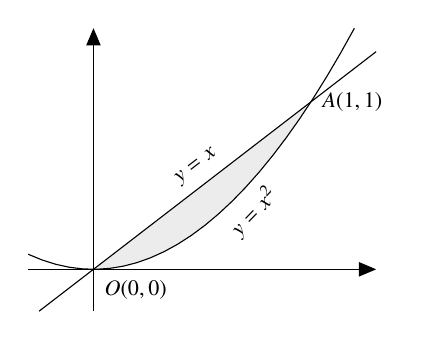
\begin{tikzpicture}
   \begin{axis}[axis lines=middle,axis line style={-triangle 45}, width=6cm, ticks=none, clip=false]
      \addplot[domain=-0.3:1.2, name path=curve, decoration={markings,mark=at position 0.5 with {\arrow{angle 90}}}]{x^2}
      node[midway, sloped, below]{$y=x^2$};
      \addplot[domain=-0.25:1.3, name path=line, decoration={markings,mark=at position 0.5 with {\arrow{angle 90}}}]{x}
      node[midway, sloped, above]{$y=x$};
      \addplot[gray,opacity=0.15] fill between[of=curve and line, soft clip={domain=0:1}];
      \node[below right] at (0,0){$O (0,0)$};
      \node[right] at (1,1){$A (1,1)$};
   \end{axis}
\end{tikzpicture}


$\begin{aligned}
   & \text{Given, }\ y=x \text{ and } y=x^2\\
   & \text{Then, } x=x^2 \\
   & \Rightarrow x-x^2 = 0 \\
   & \Rightarrow x(1-x)=0 \\
   & \therefore x = 0,1 \\
   & \therefore y = 0,1 
\end{aligned}$
\end{minipage}

\begin{tabularx}{\textwidth}{Xp{6.4cm}}
   \begin{adjustbox}{valign=t}
      $\begin{aligned}
         R.H.S
         & = \miint_S\left(\frac{\partial N}{\partial x}-\frac{\partial M}{\partial y}\right) \dx\dy \\[1ex]
         & =\mint_{x=0}^1 \mint_{y=x^2}^x\left(y^2-x\right) \dy\dx \quad = \mint_0^1\left[\frac{y^3}{3}-x y\right]_{x^2}^x \dx \\[1ex]
         & =\mint_0^1\left(\frac{x^3}{3}-x^2-\frac{x^6}{3}+x^3\right)\dx
         \quad =\mint_0^1\left(\frac{4}{3} x^3-x^2-\frac{x^6}{3}\right) \dx \\[1ex]
         & =\left[\frac{4}{3} \frac{x^4}{4}-\frac{x^3}{3}-\frac{1}{3} \frac{x^7}{7}\right]_0^1
         \quad = \frac{1}{3}-\frac{1}{3}-\frac{1}{21}-0
         \quad = -\frac{1}{21}
         \end{aligned}$
   \end{adjustbox}
   &
   \begin{adjustbox}{valign=t}
      \divideX
      $\begin{aligned}
         & \text{Here, }\\
         & M(x,y)=x y+x^2\\[1ex]
         & N(x,y)=x y^2 \\[1ex]
         & \therefore \frac{\partial N}{\partial x}=y^2\\[1ex]
         & \therefore \frac{\partial M}{\partial y}=x
      \end{aligned}$
   \end{adjustbox}
\end{tabularx}

\vspace{1ex}
Since, $L.H.S = R.H.S. \tab$ Hence, Green's Theorem has been verified.

\pagebreak

\textbf{\mred{19(b)}} Using Green's theorem evaluate
$\osint[C](x^2-2xy)\dx+(x^2y+3)\dy$,where $C$ is the closed curve of the region bounded by the $y^2=8x$ and $x=2$.

\begin{center}
   \begin{tabular}{l|l}
      \begin{adjustbox}{valign=m}
         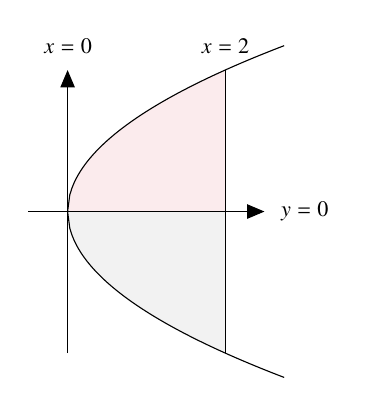
\begin{tikzpicture}
            \begin{axis}[ticks=none, axis lines=middle,axis line style={-triangle 45}, x=1cm, xmin=-0.5, xmax=2.5, ymin=-4, ymax=4, width=6cm, clip=false]
               \addplot[domain=0:2.75, samples=100, name path=C1]{sqrt(8*x)};
               \addplot[domain=0:2.75, samples=100, name path=C2]{-sqrt(8*x)};
               \addplot[name path=L1] coordinates{(0,0) (2,0) (2,4)};
               \addplot[name path=L2] coordinates{(0,0) (2,0) (2,-4)};

               \node[above=2pt] at (2,4) {$x=2$};
               \node[above=2pt] at (0,4) {$x=0$};
               \node[right=2pt] at (2.5,0) {$y=0$};

               \addplot[keyword,opacity=0.1] fill between[of=C1 and L1, soft clip={domain=0:3}];
               \addplot[gray,opacity=0.1] fill between[of=C2 and L2, soft clip={domain=0:3}];
            \end{axis}
         \end{tikzpicture}
      \end{adjustbox}
      &
      \begin{adjustbox}{valign=m}
         $\begin{array}{ll}
            M(x,y)=x^2-2xy & \tab N(x,y)=xy^2+3 \\[2ex]
            \therefore \frac{\partial N}{\partial x}=2xy &
            \therefore \frac{\partial M}{\partial y}=-2x
         \end{array}$
      \end{adjustbox}
   \end{tabular}
\end{center}

$\begin{aligned}
   & \miint_S\left(\frac{\partial^N}{\partial x}-\frac{\partial^M}{\partial y}\right) \dx\dy \\[1.5ex]
   & =\int_{x=0}^2\int_{y=\mred{-\sqrt{8x}}}^{\sqrt{8 x}}(2 x y+2 x) \dx \dy\quad
    =\mred{2}\int_{x=0}^2\int_{y=\mred{0}}^{\sqrt{8 x}}(2 x y+2 x) \dx \dy \\[1.5ex]
   & =2 \int_{x=0}^2 2 x\left[\frac{y^2}{2}+y\right]_0^{\sqrt{8 x}} \dx \quad
   =2 \int_{x=0}^2 2 x\left(\frac{8 x}{2}+\sqrt{8 x}\right) \dx \\[1.5ex]
   & =2 \int_{x=0}^2\left(8 x^2+2 \sqrt{8} x^{\frac{3}{2}}\right) \dx \quad
   =2\left[8 \frac{x^3}{3}+2 \sqrt{8} \frac{x^{\frac{5}{2}}}{\frac{5}{2}}\right]_0^2 \\[1.5ex]
   & =2\left(\frac{64}{3}+\frac{64}{5}\right) \quad
   =\frac{1024}{15}
\end{aligned}$

\pagebreak
\textbf{\mred{15(a)}} Using Green's theorem to evaluate
$\osint[c] x^2y\dx+x^2\dy$ where $C$ is the boundary described counter clockwise of the $C$ triangle with vertices $(0,0),\ (1,0),\ (1,1)$.

\Heading{Solution:}
\vspace{-1.8\baselineskip}
\begin{center}
   \begin{tabular}{lcl}
      \begin{adjustbox}{valign=t}
         $\begin{aligned}\\
            & \text{Here,}\\
            & M=x^2y \tabs\tabs N=x^2\br
            & \frac{\partial M}{\partial Y} = x^2
            \tabs\tab
            \frac{\partial N}{\partial x} = 2x\br
         \end{aligned}$   
      \end{adjustbox}
      & \divideX &
      \begin{adjustbox}{valign=t}
         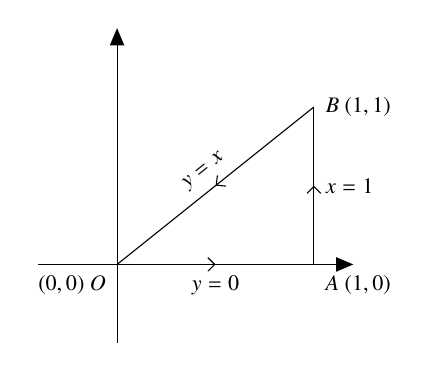
\begin{tikzpicture}[decoration={markings,mark=at position 0.5 with {\arrow{angle 90}}}]
            \draw[-triangle 45] (0,-1) -- (0,3);
            \draw[-triangle 45] (-1,0) -- (3,0);
         
            \coordinate (O) at (0,0);
            \coordinate (A) at (2.5,0);
            \coordinate (B) at (2.5,2);
         
            \draw[postaction={decorate}] (O) -- (A)
            node [below, midway] {$y=0$};
            \draw[postaction={decorate}] (A) -- (B)
            node [right, midway] {$x=1$};
            \draw[postaction={decorate}] (B) -- (O)
            node [above, midway, sloped] {$y=x$};
         
            \node[below left] at (O) {$(0,0)\ O$};
            \node[below right] at (A) {$A\ (1,0)$};
            \node[right] at (B) {$B\ (1,1)$};
         \end{tikzpicture}
      \end{adjustbox}
   \end{tabular}

   $\begin{aligned}
      & \mint_R\left(\frac{\partial N}{\partial x}-\frac{\partial M}{\partial y}\right) \dx\dy
      \quad = \mint_{x=0}^1 \ \mint_{y=0}^x\left(2 x-x^2\right) d y \dx
      \quad = \mint_0^1\left[2 x y-x^2 y\right]_0^x \dx \\[1ex]
      & =\mint_0^1\left(2 x^2-x^3\right) \dx 
      \quad = \left[\frac{2 x^3}{3}-\frac{x^4}{4}\right]_0^1
      \quad = \frac{2}{3}-\frac{1}{4}
      \tab = \frac{5}{12}
   \end{aligned}$
\end{center}

\Section{\cyan{Jacobian}}

\textbf{\mred{6(a)}} Define Jacobian of two variables. If $x=\rho \sin\theta \cos\phi$, $y=\rho \sin\theta \sin\phi$ and $z=\rho \cos\theta$ then show that $\frac{\partial\left(x,y,z\right)}{\partial\left(\rho,\theta,\phi\right)} = \rho^2\sin\theta$

\begin{tabularx}{\textwidth}{X|p{6.1cm}}
   \textbf{Jacobian of two variables:}&
   \multirow{3}{*}{
      $\begin{aligned}
         J(u,v) \ = \ 
         \frac{\partial\left(u,v\right)}{\partial\left(x,y\right)}
         \ = \ \left|\begin{array}{ll}
            \frac{\partial u}{\partial x} & \hspace{0.5em}
            \frac{\partial u}{\partial y}\\[1.5ex]
            \frac{\partial v}{\partial x} & \hspace{0.5em}
            \frac{\partial v}{\partial y}
            \end{array}\right|
      \end{aligned}$}\\
   If $u$ and $v$ are functions of two independent variable $x$ and $y$, then the determinant is known as Jacobian of $u$ and $v$ with respect to $x$ and $y$\\[-4ex]\\
\end{tabularx}

\vspace{2ex}
\Heading{Solution:}
\begin{minipage}[t]{0.46\linewidth}
\noindent
      By definition of Jacobian:\\[1ex]
      $\begin{aligned}
         |J| &=  \frac{\partial(x, y, z)}{\partial(\rho, \theta, \phi)}\\
         &= \left|\begin{array}{ccc}
            \sin\theta \cos\phi &
            \rho \cos\theta \cos\phi &
            -\rho \sin\theta \sin\phi \\[2ex]
            \sin\theta \sin\phi & 
            \rho \cos\theta \sin\phi & 
            \rho \sin\theta \cos\phi \\[2ex]
            \cos\theta & -\rho \sin\theta & 0
         \end{array}\right|
   \end{aligned}$
\end{minipage}\hspace{0.5ex}{\color{divider}\vrule width 0.35pt}\hspace{0.5ex}
\begin{minipage}[t]{0.52\linewidth}
\noindent
   Given that,\\
   $x=\rho \sin\theta \cos\phi$, \tab $y=\rho \sin\theta \sin\phi$ \tab and \tab $z=\rho \cos\theta$

   \vspace{3ex}
   \begin{tabular}{lll}
      $\frac{\partial x}{\partial \rho} = \sin\theta \cos\phi$
      &
      $\frac{\partial x}{\partial \theta} =
      \rho \cos\theta \cos\phi$
      &
      $\frac{\partial x}{\partial \phi} =
      -\rho \sin\theta \sin\phi$
      \\[2.5ex]

      $\frac{\partial y}{\partial \rho} = \sin\theta \sin\phi$
      &
      $\frac{\partial y}{\partial \theta} = 
      \rho \cos\theta \sin\phi$
      &
      $\frac{\partial y}{\partial \phi} = 
      \rho \sin\theta \cos\phi$
      \\[2.5ex]

      $\frac{\partial z}{\partial \rho} = \cos\theta$
      &
      $\frac{\partial z}{\partial \theta} = -\rho \sin\theta$
      &
      $\frac{\partial z}{\partial \phi} = 0$
   \end{tabular}
\end{minipage}

\vspace{1ex}
$\begin{aligned}
   & = \cos\theta \left[\rho^2\sin\theta\cos\theta\cos^2\phi + \rho^2\sin\theta\cos\theta\sin^2\phi\right] \tab + \tab \rho\sin\theta \left[\rho\sin^2\theta\cos^2\phi+\rho\sin^2\theta\sin^2\phi\right] \tab + 0 \\[1ex]
   & = \cos\theta \left[\rho^2\sin\theta\cos\theta
   \left(\cos^2\phi + \sin^2\phi\right)
   \right] \tab + \tab \rho\sin\theta \left[\rho\sin^2\theta
   \left(\cos^2\phi + \sin^2\phi\right)
   \right]\\[1ex]
   & = \rho^2\sin\theta\cos^2\theta + \rho^2\sin^3\theta
   \tab = \rho^2\sin\theta \left(\cos^2\theta + \sin^2\theta\right)
   \tab = \rho^2\sin\theta
\end{aligned}$

\pagebreak
\Heading{Jacobian of $n$ variables:}
If $u_1,\ u_2,\ldots u_n$ are $n$ functions of $n$ variables $x_1,\ x_2,\ \ldots x_n$.\\
Then the determinant,
$$
\left|\begin{array}{llll}
\frac{\partial u_1}{\partial x_1}, \hspace{0.5em}
\frac{\partial u_1}{\partial x_2}, & \ldots &
\frac{\partial u_1}{\partial x_n}\\[2ex]
\frac{\partial u_2}{\partial x_1}, \hspace{0.5em}
\frac{\partial u_2}{\partial x_2}, & \ldots &
\frac{\partial u_2}{\partial x_n}\\[2ex]
\frac{\partial u_3}{\partial x_1}, \hspace{0.5em}
\frac{\partial u_3}{\partial x_2}, & \ldots &
\frac{\partial u_n}{\partial x_n}
\end{array}\right|
$$

is called the Jacobian of $u_1,\ u_2,\ \ldots u_n$ with respect to $x_1,\ x_2\ \ldots x_n$ and denoted by $J\left(u_1, u_2, \ldots u_n\right)$ or
$\frac{\partial\left(u_1, u_2 \ldots u_n\right)}{\partial\left(x_1, x_2, \cdots x_n\right)}$

\vspace{4ex}
\textbf{\mred{14.}} Evaluate the $\miint_R \frac{x-y}{x+y} \,dA$ where $R$ is the region enclosed by the lines \ $x-y=0, \ x-y=1, \ x+y=1, \ x+y=3$.

\Heading{Solution:}
Let, $u=x-y$ and $v=x+y$ \ then $x y$ plane corresponds to the $uv$ plane. $u=0, \ u=1, \ v=1, \ v=3$

\vspace{-\baselineskip}
\begin{center}
   \begin{tabular}{ccc}
      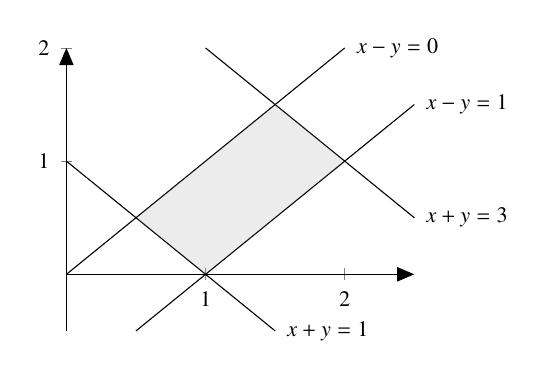
\begin{tikzpicture}
         \begin{axis}[axis lines=middle,axis line style={-triangle 45}, width=6cm, clip=false]
            \addplot[domain=0:2, name path=A]{x}
            node[right]{$x-y=0$};
            \addplot[domain=0:1.5, name path=B]{1-x}
            node[right]{$x+y=1$};
            \addplot[domain=0.5:2.5, name path=C]{x-1}
            node[right]{$x-y=1$};
            \addplot[domain=1:2.5, name path=D]{3-x}
            node[right]{$x+y=3$};

            \path[name intersections={of=A and B,by=AB}];
            \path[name intersections={of=B and C,by=BC}];
            \path[name intersections={of=C and D,by=CD}];
            \path[name intersections={of=D and A,by=DA}];
      
            \fill[gray,opacity=0.15] (AB) -- (BC) -- (CD) -- (DA) -- cycle;
         \end{axis}
      \end{tikzpicture}
      &\tab  \tab&
      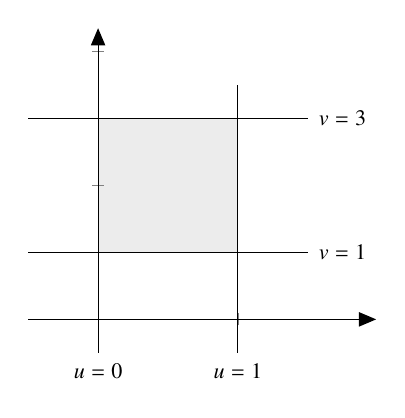
\begin{tikzpicture}
         \begin{axis}[axis lines=middle,axis line style={-triangle 45}, y=0.85cm, xmax=1.99, ymax=4.35, width=6cm, xticklabels={}, yticklabels={}, clip=false]
            \fill[gray, opacity=0.15] (0,1) rectangle (1,3);
            \addplot[domain=-0.5:1.5]{0};
            \addplot[domain=-0.5:1.5]{1}
            node[right]{$v=1$};
            \addplot[domain=-0.5:1.5]{3}
            node[right]{$v=3$};
            \draw (0,3.5) -- (0,-0.5)
            node[below]{$u=0$};
            \draw (1,3.5) -- (1,-0.5)
            node[below]{$u=1$};
         \end{axis}
      \end{tikzpicture}\\
      $xy$ plane & & $uv$ plane
   \end{tabular}   
\end{center}

\begin{minipage}[t]{0.61\linewidth}
\noindent
   \begin{adjustbox}{valign=t}
      $\begin{aligned}
         & \therefore \miint_R \frac{x-y}{x+y} dA
         \quad = \mint_{u=0}^1 \mint_{v=1}^3 \frac{u}{v} \left| J \right| \dv\du
         \quad =\mint_{u=0}^1 \mint_{v=1}^3 \frac{u}{v} \frac{1}{2} \dv\du\\[1ex]
         & =\frac{1}{2} \mint_{u=0}^1 \mint_{v=1}^3 \frac{1}{v}\dv \cdot u\du
         \quad =\frac{1}{2} \mint_{u=0}^1 \left[\ln v\right]_1^3 u\du
         \quad =\frac{1}{2} \mint_0^1(\ln 3-\ln 1) u\du\\[1ex]
         & =\frac{1}{2}(\ln 3-0)\left[\frac{u^2}{2}\right]_0^1
         \quad =\frac{1}{2} \ln 3\left(\frac{1}{2}-0\right)\ =\frac{1}{4} \ln 3
      \end{aligned}$
   \end{adjustbox}
\end{minipage}\hspace{0.5ex}{\color{divider}\vrule width 0.35pt}\hspace{0.5ex}
\begin{minipage}[t]{0.37\linewidth}
\noindent
   % \begin{adjustbox}{valign=t}
   %    $\begin{array}{ll}
   %       u=x-y & u=x-y \\
   %       v=x+y & v=x+y \\
   %       \hline u+v=2x & u-v=-2y \\[1ex]
   %       \therefore x=\frac{u+v}{2} & \therefore y=\frac{u-v}{-2}
   %    \end{array}$
   % \end{adjustbox}

   %    \vspace{2ex}
   %    \begin{tabular}{ll}
   %       $\frac{\partial x}{\partial u}=\frac{1}{2}$ & \hspace{0.5em}
   %       $\frac{\partial x}{\partial v}=\frac{1}{2}$ \\[2ex]
   %       $\frac{\partial y}{\partial u}=-\frac{1}{2}$ & \hspace{0.5em}
   %       $\frac{\partial y}{\partial v}=\frac{1}{2}$
   %    \end{tabular}
      
   %    \vspace{2ex}
   %    $\begin{aligned}
   %       \left| J \right| = 
   %    \frac{\partial\left(x,y\right)}{\partial\left(u,v\right)} &=
   %    \left|\begin{array}{rr}
   %       \frac{1}{2} &\hspace{0.25em} \frac{1}{2} \\[2ex]
   %       -\frac{1}{2} &\hspace{0.25em} \frac{1}{2}
   %    \end{array}\right| =\frac{1}{4}+\frac{1}{4}=\frac{1}{2}
   %    \end{aligned}$

      % \vspace{4ex}
      $u=x-y \tabs v=x+y$

      \vspace{2ex}
      \begin{tabular}{ll}
         $\frac{\partial u}{\partial x}=1$ & \hspace{0.5em}
         $\frac{\partial u}{\partial y}=-1$ \\[2ex]
         $\frac{\partial v}{\partial x}=1$ & \hspace{0.5em}
         $\frac{\partial v}{\partial y}=1$
      \end{tabular}

      \vspace{2ex}
      $\begin{aligned}
         \left| J^{\prime} \right| = 
      \frac{\partial\left(u,v\right)}{\partial\left(x,y\right)} &=
      \left|\begin{array}{rr}
         1 &\hspace{0.25em} -1 \\[2ex]
         1 &\hspace{0.25em} 1
      \end{array}\right| =1+1=2
      \end{aligned}$

      \vspace{2ex}
      $|J| = \frac{1}{|J^{\prime}|} = \frac{1}{2}$
\end{minipage}

\pagebreak
\textbf{\mred{16(b)}} Evaluate the $\miint_R e^{x y} \,dA$ where $R$ is the region enclosed by the lines $y=\frac{1}{2}x,\ \ y=x$ and the hyperbolas $y=\frac{1}{x}$ and $y=\frac{2}{x}$.

\Heading{Solution:}
\vspace{1ex}
\begin{tabular}{lclcl}
   \begin{adjustbox}{valign=t}
      $\begin{aligned}
         & y = \frac{1}{2}x \tab \Rightarrow \frac{y}{x} = \frac{1}{2}\\
         & y = x \tab \Rightarrow \frac{y}{x} = 1\\
         & \text{Also, }\\
         & y=\frac{1}{x} \tab \Rightarrow xy=1\\
         & y=\frac{2}{x} \tab \Rightarrow xy=2
      \end{aligned}$
   \end{adjustbox}
   &\tab \divideX \ &
   \begin{adjustbox}{valign=t}
      $\begin{aligned}
         &\text{Let } u=\frac{y}{x} \text{ \tab and \tab } v=xy\\[2ex]
         &\begin{array}{ll}
            \frac{\partial u}{\partial x}=\frac{-y}{x^2} & \tabs
            \frac{\partial u}{\partial y}=\frac{1}{x}\\[2ex]
            \frac{\partial v}{\partial x}=y & \tabs
            \frac{\partial v}{\partial y}=x
         \end{array}
      \end{aligned}$
   \end{adjustbox}
   &\tab \divideX &
   \begin{adjustbox}{valign=t}
      $\begin{aligned}
         \left|J^{\prime}\right| \ = \ 
         \frac{\partial(u,v)}{\partial(x,y)} &= 
         \left|\begin{array}{ll}
            \frac{\partial u}{\partial x}&
            \frac{\partial u}{\partial y} \\[1ex]
            \frac{\partial v}{\partial x}&
            \frac{\partial v}{\partial y}
         \end{array}\right|
         \ = \ \left|\begin{array}{cc}
            \frac{-y}{x^2} & \frac{1}{x} \\ y & x
         \end{array}\right| &&\\[1ex]
         & = -\frac{y}{x}-\frac{y}{x} \ = \ -\frac{2 y}{x}=-2u &&\\[1ex]
         \therefore |J| = \frac{1}{|J^\prime|} = \frac{1}{-2u}
         & \tabs \tabs \left[\ \because |J|\cdot|J^\prime| =1\ \right] &&\\
      \end{aligned}$
   \end{adjustbox}
\end{tabular}

\vspace{2ex}
Now,\\
$\begin{aligned}
\miint_R e^{x y} \,dA
\quad & =\mint_{u=\frac{1}{2}}^1 \mint_{v=1}^2 e^v \ |J| \,\dv\du
\quad =\mint_{u=\frac{1}{2}}^1 \mint_{v=1}^2 e^v \ \frac{-1}{2u} \,\dv\du
\quad =\mint_{u=\frac{1}{2}}^1 \left[e^v\right]_1^2 \ \frac{-1}{2u} \du \\[1ex]
& =-\frac{1}{2} \int_{\frac{1}{2}}^1\left(e^2-e^1\right) \ \frac{1}{u}\du
\quad = -\frac{1}{2}\left(e^2-e\right) \ [\ln u]_{\frac{1}{2}}^1 \\[1ex]
& =-\frac{1}{2}\left(e^2-e\right)\left(\ln 1-\ln \frac{1}{2}\right)
\quad =-\frac{1}{2}\left(e^2-e\right)\left(\ln 1- (\ln 1 - \ln 2)\right)\\[1ex]
& =-\frac{1}{2}\left(e^2-e\right) \ln{2}
\end{aligned}$


\pagebreak
\Section{\cyan{Gauss Divergence Theorem}}
\textbf{Gauss Theorem:} The surface integral of the normal component of a continuous diffentiable vector $\vec{F}$ taken over a closed surface $S$ is equal to the integral of the divergence of $\vec{F}$ taken over the volume $V$ enclosed by the surface.

\vspace{-\baselineskip}
\begin{center}
   $\text { Mathematically } \miint_S \left(\vec{F} \cdot \vec{n}\right) \dS =\miiint_V \left(\nabla \cdot \vec{F}\right) \,dV$\\[1.5ex]
   where $n$ is the positive normal to $s$.
\end{center}


\textbf{\mred{16(a)}} Use Divergence theorem to evaluate
$ \miint_S \overline{F}.\ \overline{n} \dS$ where $\vec{F} = 4x\vec{i} - 2y^2 \vec{j}+ z^2 \vec{k}$ and $S$ is the surface bounded by the
$S$ region $x^2+y^2=4,\ \ z=0$\ \ and \ $z=3$.




\Heading{Solution:}
Here,\\[1ex]

\vspace{-\baselineskip}
\begin{tabularx}{\textwidth}{X|p{3.25cm}p{4cm}}
   \begin{adjustbox}{valign=t}
      $\nabla \cdot \vec{F}=\frac{\partial}{\partial x}(4x)-\frac{\partial}{\partial y}\left(2 y^2\right)+\frac{\partial}{\partial z} \left(z^2\right) \quad = 4-4y+2z$
   \end{adjustbox}
   &
   \begin{adjustbox}{valign=t}
      $\begin{aligned}
         & \text {Here, } \\
         & x^2+y^2=4 \\
         & \Rightarrow y= \pm \sqrt{4-x^2} \\
      \end{aligned}$
   \end{adjustbox}
   &
   \begin{adjustbox}{valign=t}
      $\begin{aligned}
         & \text {Also, } \\
         & x^2=4 \\
         & \Rightarrow x= \pm 2
      \end{aligned}$
   \end{adjustbox}
\end{tabularx}

\vspace{2ex}
$\begin{aligned}
   \therefore \text { R.H.S }
   = \miiint_v \nabla \cdot \F \ \,dV
   &=\mint_{x=-2}^2 \ \mint_{y=-\sqrt{4-x^2}}^{\sqrt{4-x^2}} \ \mint_{z=0}^3 4-4y+2z \ \dz\dy\dx 
   \quad =\int_{-2}^2 \ \int_{-\sqrt{4-x^2}}^{\sqrt{4-x^2}} \ \left[4 z-4 y z+2 \frac{z^2}{2}\right]_0^3 \dy\dx \\[1ex]
   & =\int_{-2}^2 \ \int_{-\sqrt{4-x^2}}^{\sqrt{4-x^2}}
   \left(12-12 y+9-0\right) \ \dy\dx
   \quad =\int_{-2}^2  \ \int_{-\sqrt{4-x^2}}^{\sqrt{4-x^2}}
   \left(21-12y\right) \ \dy\dx \\[1ex]
   & =\int_{-2}^2\left[21 y-12 \frac{y^2}{2}\right]_{-\sqrt{4-x^2}}^{\sqrt{4-x^2}} \ \dx 
   \quad =\int_{-2}^2\left[21y - 6y^2\right]_{-\sqrt{4-x^2}}^{\sqrt{4-x^2}} \ \dx\\[1ex]
   & =\int_{-2}^2\left[21\left(\sqrt{4-x^2}+\sqrt{4-x^2}\right)-6\left(\left(\sqrt{4-x^2}\right)^2 - \left(-\sqrt{4-x^2}\right)^2\right)\right] \dx \\[1ex]
   & =\int_{-2}^2\left[21\left(2\sqrt{4-x^2}\right)-6\left((4-x^2) - (4-x^2)\right)\right] \dx \\[1ex]
   & =\int_{-2}^2\left[21\left(2\sqrt{4-x^2}\right)-6\left(4-x^2 - 4+x^2\right)\right] \dx 
   \quad =42 \int_{-2}^2 \sqrt{4-x^2} \ \dx\\[1ex]
   & =42\left[\frac{x \sqrt{4-x^2}}{2}+\frac{4}{2} \sin ^{-1} \frac{x}{2}\right]_{-2}^{2} \tabs\tabs
   \left[\because \int \sqrt{a^2-x^2} = \frac{x \sqrt{a^2-x^2}}{2}+\frac{a^2}{2} \sin^{-1} \frac{x}{a}+C\right]\\[1ex]
   & =42\left[0+2 \sin ^{-1}(1)-0-2 \sin ^{-1}(-1)\right] \tab =42 \cdot\left[2 \cdot \frac{\pi}{2}+2 \cdot \frac{\pi}{2}\right] \tab = 84 \pi \\
\end{aligned}$

\pagebreak


\begin{minipage}[t]{0.7\linewidth}
\noindent
   \begin{adjustbox}{valign=t}
      $\therefore \text {L.H.S }
   = \miint_S \vec{F}.\ \vec{n} \ \dS
   = \miint_{\substack{S1\\[0.25ex](z=0)}}
      \vec{F}.\ \vec{n} \ \,dS_1 +
      \miint_{\substack{S2\\[0.25ex](z=3)}}
      \vec{F}.\ \vec{n} \ \,dS_2 +
      \miint_{\substack{S3\\[0.25ex](x^2+y^2=4)}}
      \vec{F}.\ \vec{n} \ \,dS_2$
   \end{adjustbox}

   \vspace{2ex}
   \textbf{On \mred{$\mathbf{S_1}:$}}
   $\begin{array}{llcl}
      z=0 & n=\vec{k} &\tab& \therefore \vec{F} \cdot \vec{n}=z^2=0
   \end{array}$ \tabs
   $\therefore \miint_{S1}\vec{F}.\ \vec{n} \ \,dS_1 = 0$
\end{minipage}
\begin{minipage}[t]{0.28\linewidth}
\noindent
   \begin{adjustbox}{valign=t}
      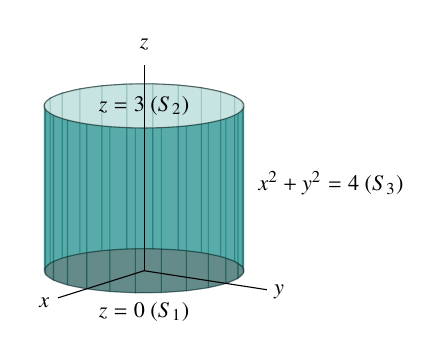
\begin{tikzpicture}
         \begin{axis}[
            smooth, hide axis,
            view={125}{15},
            axis lines=center,
            width=6cm,
            ticks=none,
            clip=false
         ]
            % Curved surace
            \addplot3 [surf,domain=0:360, y domain=0:4, samples y= 2, colormap/viridis, opacity=0.5]({cos(x)}, {sin(x)}, {y});
      
            % Top surface
            \addplot3[domain=0:360,samples=100,samples y=0,fill=white, opacity=0.5]({cos(x)}, {sin(x)}, 4);
      
            % Bottom surface
            \addplot3[domain=0:360,samples=100,samples y=0,fill=black, opacity=0.3]({cos(x)}, {sin(x)}, 0);
      
            \node at (0,0,-1) {$z=0\ (S_1)$};
            \node at (0,0,4) {$z=3\ (S_2)$};
            \node[right] at (0,1.25,2.5) {$x^2+y^2=4\ (S_3)$};
            \node at (1.75,0,0) {$x$};
            \node at (0,1.65,0) {$y$};
            \node at (0,0,5.5) {$z$};
      
            % Axis
            \addplot3[mark=none, color=black] coordinates {(0,0,0) (1.5,0,0)};
            \addplot3[mark=none, color=black] coordinates {(0,0,0) (0,1.5,0)};
            \addplot3[mark=none, color=black] coordinates {(0,0,0) (0,0,5)};
         \end{axis}
      \end{tikzpicture}
   \end{adjustbox}  
\end{minipage}

\textbf{On \mred{$\mathbf{S_2}:$}}\\[1ex]
\begin{tabularx}{\textwidth}{X|X}
   $\begin{aligned}
      &\begin{array}{llcl}
         z=3 & n=\vec{k} &\tab& \therefore \vec{F} \cdot \vec{n}=z^2=3^2=9
      \end{array}\\[1ex]
      &\therefore \miint_{S2}\vec{F}.\ \vec{n} \ \,dS_2 = \miint_{S2} 9 \,dS_2 = 9 \times 4\pi = 36\pi
   \end{aligned}$
   &
   $\begin{aligned}
      & \text{Here, }
      \ x^2+y^2=4 \tabs \therefore r=2\\
      & \text{Area of }
      S_2=\pi r^2 \ =\pi(2)^2 \ =4 \pi
   \end{aligned}$
\end{tabularx}


\vspace{1ex}

\textbf{On \mred{$\mathbf{S_3}:$}} $x^2+y^2-4=0$

\begin{tabularx}{\textwidth}{X|X}
   $\begin{aligned}
      &\begin{aligned}
         \therefore \vec{F}.\ \vec{n} & =\left(4x\vec{i} - 2y^2 \vec{j}+ z^2 \vec{k}\right) \cdot\left(\frac{x}{2} \vec{i}+\frac{y}{2} \vec{j}\right) \\
         & =2x^2-y^3+0
      \end{aligned}\\[2ex]
      & \therefore \miint_{S3}\vec{F}.\ \vec{n} \ \,dS_3 =
      \miint_{S3}\left(2x^2-y^3\right) \ \,dS_3
   \end{aligned}$
   &
   $\begin{aligned}
      & \nabla(x^2+y^2-4)=2x\vec{i} + 2y\vec{j}\\[1ex]
      & \begin{aligned}
            \therefore \vec{n} & =
            \frac{2x\vec{i} + 2y\vec{j}}{\sqrt{(2x)^2+(2y)^2}}
            \tab =\frac{2x\vec{i} + 2y\vec{j}}{\sqrt{4\left(x^2+y^2\right)}} \\[1ex]
            & =\frac{2x\vec{i} + 2y\vec{j}}{\sqrt{16}}
            \tab =\frac{x}{2} \vec{i}+\frac{y}{2} \vec{j}
      \end{aligned}\\[2ex]
   \end{aligned}$
\end{tabularx}


\vspace{-0.5\baselineskip}
\begin{tabularx}{\textwidth}{Xp{5cm}}
   \begin{adjustbox}{valign=t}
      $\begin{aligned}
         \hspace{7em}
         & = \mint_{\theta=0}^{2\pi} \ \mint_{z=0}^{3} 2(2\cos\theta)^2-(2\sin\theta)^3 \ \ 2\dtheta\dz\\
         & =2 \int_{0}^{2\pi} [z]_0^3\left(8 \cos^2 \theta-8 \sin ^3 \theta\right) \dtheta \\
         & =2 \int_{0}^{2\pi} 3\left(8 \cos^2 \theta-8 \sin ^3 \theta\right) \dtheta \\
         & =6 \int_0^{2 \pi} 4\cdot 2 \cos^2{\theta} \dtheta 
         \ \ -6 \int_0^{2\pi} 2\cdot 4 \sin^3{\theta} \dtheta \\
         & =24 \int_0^{2 \pi}(\ul{$1+\cos 2 \theta$}) d \theta-12 \int_0^{2 \pi}(\ul{$3 \sin \theta-\sin 3 \theta$}) d \theta \\
         & =24\left[\theta+\frac{\sin 2 \theta}{2}\right]_0^{2 \pi}-12\left[-3 \cos \theta+\frac{\cos 3 \theta}{3}\right]_0^{2 \pi} \\
         & =24[2 \pi+0-0]-12\left[-3.1+\frac{1}{3}+3-\frac{1}{3}\right] \tab = 48 \pi \\
      \end{aligned}$
   \end{adjustbox}
   & 
   \begin{adjustbox}{valign=t}
      \divideX
      $\begin{aligned}
         & \text{Let, }\\
         & x = r\cos\theta = 2\cos\theta\\
         & y = r\sin\theta = 2\sin\theta\\
         & z = z\\
         & \therefore dS_3 = 2\dtheta\,dz\\[3ex]
         & \text{Formula},\\
         & 2 \cos^2{\theta} = 1+\cos 2 \theta\\
         & 4 \sin^3{\theta} = 3 \sin \theta-\sin 3 \theta
      \end{aligned}$
   \end{adjustbox}
\end{tabularx}

$\begin{aligned}
   \therefore \miint_S \vec{F}.\ \vec{n} \ \dS
   & = \miint_{S1}\vec{F}.\ \vec{n} \ \,dS_1 +
      \miint_{S2}\vec{F}.\ \vec{n} \ \,dS_2 +
      \miint_{S3}\vec{F}.\ \vec{n} \ \,dS_2\\
   & = 0 \ + \ 36\pi \ + \ 48\pi\ = 84\pi=\text { R.H.S \ (verified)}
\end{aligned}$

 
\pagebreak
\Section{\cyan{Stoke's theorem}}

\textbf{Stoke's theorem:} If the components of a vector field $\vec{F}(x,y,z) = f(x,y,z)\vec{i}+g(x,y,z)\vec{j}+h(x,y,z)\vec{k}$ are continuous and have continuous first partial derivatives on some open set $S$ and $C$ be smooth closed curve then, $$\osint[C]\vec{F} \cdot \dvr = \miint_S(\nabla\times\F) \cdot \vec{n} \dS$$
relationship between line and surface integrals a generalization of Green's theorem to three dimensions is called Stoke's theorem.

\textbf{\mred{Exr.}} Verify stoke's theorem for the function $\F=x^2\i + xy\j$ taken round the square in the plane $z=0$ whose sides are along the lines $x=0,\ y=0$

\Heading{Solution:}
\begin{minipage}[t]{0.66\linewidth}
\noindent
\begin{adjustbox}{valign=t}
   $\begin{aligned}
      \text{L.H.S } = \osint[C]\vec{F} \cdot \dvr \tab
      & = \mint_{OABCO} x^2\dx + xy\dy\\[1ex]
      & = 
      \mint_{\substack{OA \br y=0 \br dy=0}} x^2\dx+
      \mint_{\substack{AB \br x=a \br dx=0}} ay\dy+
      \mint_{\substack{BC \br y=a \br dy=0}} x^2\dx+
      \mint_{\substack{CO \br x=0 \br dx=0}} 0\\[1ex]
      & = \int_0^a x^2\dx+ \int_0^a ay\dy+ \int_a^0 x^2\dx + \int 0\\[1ex]
      & = \left[\frac{x^3}{3}\right]_0^a + \left[\frac{ay^2}{2}\right]_0^a+\left[\frac{x^3}{3}\right]_a^0 + 0\\[1ex]
      & = \frac{a^3}{3}+\frac{a^3}{2}-\frac{a^3}{3} \tabs = \frac{a^3}{2}
   \end{aligned}$
\end{adjustbox}
\end{minipage}\hspace{0.5ex}{\color{divider}\vrule width 0.35pt}\hspace{0.5ex}
\begin{minipage}[t]{0.32\linewidth}
\noindent
   \begin{adjustbox}{valign=t}
      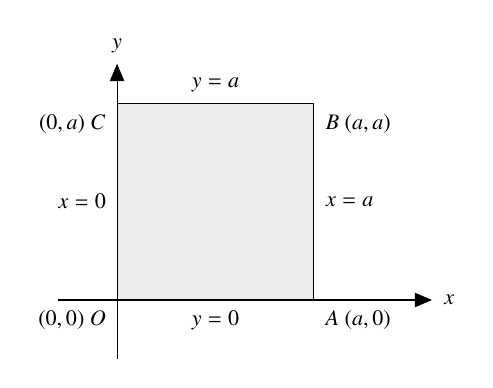
\begin{tikzpicture}
         \draw[-triangle 45] (0,-0.75) -- (0,3) node[above]{$y$};
         \draw[-triangle 45] (-0.75,0) -- (4,0) node[right]{$x$};

         \coordinate (O) at (0,0);
         \coordinate (A) at (2.5,0);
         \coordinate (B) at (2.5,2.5);
         \coordinate (C) at (0,2.5);
         
         \fill[gray, opacity=0.15] (O) rectangle (B);
         \draw
         (O) --
         (A) node[midway, below]{$y=0$} --
         (B) node[midway, right]{$x=a$} --
         (C) node[midway, above]{$y=a$} --
         (O) node[midway, left]{$x=0$};

         \node[below left] at (O) {$(0,0)\ O$};
         \node[below right] at (A) {$A\ (a,0)$};
         \node[below right] at (B) {$B\ (a,a)$};
         \node[below left] at (C) {$(0,a)\ C$};
      \end{tikzpicture}
   \end{adjustbox}
   
   \vspace{2ex}
   $\begin{aligned}
      & \text{Here, } \\
      & \F=x^2\i + xy\j \text{ \ \ and \ \ } \r = x\i + y\j\\
      &\therefore \dvr = \dx\i + \dy\j\\
      &\therefore \F.\ \dvr = x^2\dx + xy\dy\\
   \end{aligned}$
\end{minipage}

\vspace{2ex}
\begin{minipage}[t]{0.66\linewidth}
\noindent
   \begin{adjustbox}{valign=t}
      $\begin{aligned}
         \text{R.H.S}
         = \miint_R (\nabla\times\F) \cdot \vec{n}\dS \tab
         & = \miint_S y\k \cdot \vec{k}\dS \tab
         = \int_{y=0}^a\int_{x=0}^a y\dx\dy\\[1ex]
         & = \int_{y=0}^a \left[x\right]_0^a y\dy \tab
         = \int_{y=0}^a ay \dy \tab
         = a\left[\frac{y^2}{2}\right]_0^a\\[1ex]
         & = a\cdot\frac{a^2}{2} \tab
         = \frac{a^3}{2}\\
         & = \text{L.H.S  \tabs (verified)}
      \end{aligned}$
   \end{adjustbox}
\end{minipage}\hspace{0.5ex}{\color{divider}\vrule width 0.35pt}\hspace{0.5ex}
\begin{minipage}[t]{0.32\linewidth}
\noindent
   \begin{adjustbox}{valign=t}
      $\begin{aligned}\\
         & \nabla \times \F  =
            \left|\begin{array}{ccc}
               \i & \j & \k \\[1ex]
               \pp[x]{} & \pp[y]{} & \pp[z]{}\\
               x^2 & xy & 0
            \end{array}\right|\\
         & = \i(0-0)-\j(0-0)+\k(y-0)\\
         & = y\k
      \end{aligned}$
   \end{adjustbox}
\end{minipage}

\pagebreak
\textbf{\mred{20(a)}} Using Stoke's theorem or otherwise evaluate $\osint[C]\vec{F} \cdot \dvr$ where $\F=(x^2+y^2)\i-2xy\j$ taken round the rectangle bounded by the lines $x=\pm a,\ y=0,\ y=b$.


\Heading{Solution:}
\begin{minipage}[t]{0.64\linewidth}
   \noindent
      \begin{adjustbox}{valign=t}
         $\begin{aligned}
            \miint_R (\nabla\times\F) \cdot \vec{n}\dS & = \miint_S -4y\k \cdot \vec{k}\dS \tab\\[1ex]
            & = \int_{y=0}^b\int_{x=-a}^a -4y\dx\dy \\[1ex]
            & = -4 \int_{y=0}^b y\dy \int_{x=-a}^a \dx\\[1ex]
            & = -4 \cdot \left[\frac{y^2}{2}\right]_{0}^b \cdot \left[x\right]_{-a}^a \\[1ex]
            & = -4 \cdot \frac{b^2}{2} \cdot (a+a)\\[1ex]
            & = -4 \cdot \frac{b^2}{2} \cdot 2a \quad = -4ab^2
         \end{aligned}$
      \end{adjustbox}
   \end{minipage}\hspace{0.5ex}{\color{divider}\vrule width 0.35pt}\hspace{0.5ex}
   \begin{minipage}[t]{0.34\linewidth}
   \noindent
      \begin{adjustbox}{valign=t}
         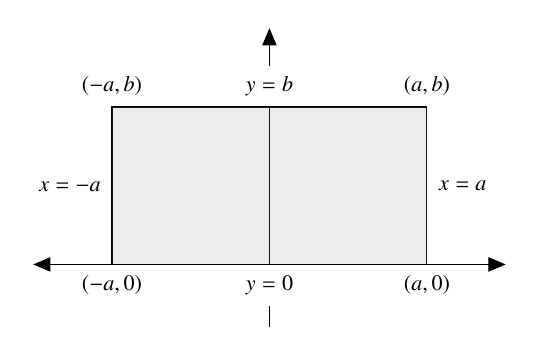
\begin{tikzpicture}
            \draw[-triangle 45] (0,-0.8) -- (0,3);
            \draw[triangle 45-triangle 45] (-3,0) -- (3,0);
         
            \coordinate (A) at (-2,2);
            \coordinate (B) at (2,2);
            \coordinate (C) at (2,0);
            \coordinate (D) at (-2,0);
         
            \node[above] at (A) {$(-a,b)$};
            \node[above] at (B) {$(a,b)$};
            \node[below] at (C) {$(a,0)$};
            \node[below] at (D) {$(-a,0)$};
         
            \draw (D) --
            (A) node[midway, left]{$x=-a$} --
            (B) node[midway, above, fill=white]{$y=b$} --
            (C) node[midway, right]{$x=a$} --
            (D) node[midway, below, fill=white]{$y=0$};
         
            \fill[gray, opacity=0.15] (A) rectangle (C);
         \end{tikzpicture}
      \end{adjustbox}

      $\begin{aligned}\\
         & \nabla \times \F  =
            \left|\begin{array}{ccc}
               \i & \j & \k \\[1ex]
               \pp[x]{} & \pp[y]{} & \pp[z]{}\\
               x^2+y^2 & -2xy & 0
            \end{array}\right|\\
         & = \i(0-0)-\j(0-0)+\k(-2y-2y)\\
         & = -4y\k
      \end{aligned}$
   \end{minipage}
\pagebreak
\Section{Coordinate System}

\vspace{1ex}
\begin{tabularx}{\textwidth}{p{5cm}|X}
   \begin{tabular}{ll}
      Cartesian &: $(x,y)$ \\
      Polar &: $(r,\theta)$ \\
      Rectangular &: $(x,y,z)$ \\
      Cylindrical &: $(\rho,\phi,z)$ \\
      Spherical &: $(r,\theta,\phi)$ \\
   \end{tabular}
   &
   $\begin{array}{l|l|l}
      \text{Cartesian -- Polar} &
      \text{Rectangular -- Cylindrical} &
      \text{Rectangular -- Spherical}\\
      x=r\cos\theta & x=\rho\cos\phi & x=r\sin\theta\cos\phi\\
      y=r\sin\theta & y=\rho\sin\phi & y=r\sin\theta\sin\phi\\
      & z=z & z=r\cos\theta\\
      |J| = r \dtheta\dz & |J| = \rho\ \drho\dphi\dz & |J| = r^{2}\sin\theta \dr\dtheta\dphi
   \end{array}$
\end{tabularx}

\vspace{4ex}
\textbf{\mred{Exr.}} Use triple integration in cylindrical coordinates to find the volume of the solid $G$ that is bounded above by the hemisphere \ $Z=\sqrt{25-x^2-y^2}$, \ below by $xy$-plane and laterally by the cylinder $x^2+y^2=9$

\Heading{Solution:}
\begin{tabularx}{\textwidth}{p{1.9cm}|p{4.5cm}|X|p{2.9cm}}
   $\begin{aligned}
      & x=\rho \cos \phi \\
      & y=\rho \sin \phi \\
      & z=z
   \end{aligned}$
   &
   $\begin{aligned}
      & x^2+y^2=9 \\
      & \Rightarrow \rho^2 (\cos^2 \phi+\sin^2 \phi) =9 \\
      & \Rightarrow \rho= \pm 3
   \end{aligned}$
   &
   $\begin{array}{rl}
      \text{Here, the upper surface } \ z &=\sqrt{25-x^2-y^2}\\
      & =\sqrt{25-\rho^2} \\
      \text{the lower surface } \ z &=0
   \end{array}$
   &
   $\begin{aligned}
      dV & = \dx\dy\dz \\
      & =|J| \ \drho\dphi\dz \\
      & =\rho \ \drho\dphi\dz \\
   \end{aligned}$
\end{tabularx}


   % $\begin{array}{lll}
   %    \text{Here, } & \text{the upper surface } &
   %    z=\sqrt{25-x^2-y^2}=\sqrt{25-\rho^2} \\
   %    & \text{the lower surface } & z=0
   % \end{array}$

   % \vspace{2ex}
   % Put, $x=\rho \cos \phi \quad y=\rho \sin \phi \quad z=\sqrt{25-\rho^2}$

   % $x^2+y^2=9 \quad
   % \Rightarrow \rho^2 (\cos^2 \phi+\sin^2 \phi)=9 \tab
   %  \Rightarrow \rho^2=9 \tab \therefore \rho= \pm 3$

\begin{center}
   $\begin{aligned}
      |J| = \pp[(\rho,\phi,z)]{(x,y,z)} =
      \left|\begin{array}{lll}
         \frac{\partial x}{\partial \rho} & \frac{\partial x}{\partial \phi} & \frac{\partial x}{\partial z} \\
         \frac{\partial y}{\partial \rho} & \frac{\partial y}{\partial \phi} & \frac{\partial y}{\partial z} \\
         \frac{\partial z}{\partial \rho} & \frac{\partial z}{\partial \phi} & \frac{\partial z}{\partial z}
      \end{array}\right| &=
      \left|\begin{array}{ccc}
         \cos \phi & -\rho \sin \phi & 0 \\
         \sin \phi & \rho \cos \phi & 0 \\
         0 & 0 & 1
      \end{array}\right| \tab
      & =\rho\left(\cos^2 \phi+\sin^2 \phi\right) =\rho
   \end{aligned}$
\end{center}

\begin{minipage}[t]{0.66\linewidth}
\noindent
   \begin{adjustbox}{valign=t}
      $\begin{aligned}
         \text{Volume } v=\miiint_G \,dV
         & =\int_{\phi=0}^{2 \pi} \int_{\rho=0}^3 \int_{z=0}^{\sqrt{25-\rho^2}} \rho \ \dz\drho\dphi \\[1ex]
         & =\int_0^{2 \pi} \int_0^3 \left[z\right]_0^{\sqrt{25-\rho^2}} \ \rho  \drho\dphi \\[1ex]
         & =\int_0^{2 \pi} \int_0^3 \sqrt{25-\rho^2} \ \rho  \drho\dphi \\[1ex]
         & =\int_0^{2 \pi} \int_{25}^{16} \sqrt{y} \ \frac{dy}{-2} \ \dphi 
         \quad =\int_{\phi=0}^{2 \pi} \dphi \int_{y=25}^{16} \sqrt{y} \ \frac{dy}{-2}\\[1ex]
         & = \int_{\phi=0}^{2 \pi} \dphi
         \cdot -\frac{1}{2}\int_{y=25}^{16} y^{\frac{1}{2}} \dy \quad
         = \left[\phi\right]_{0}^{2 \pi} \cdot -\frac{1}{2}
          \left[\frac{y^{\frac{3}{2}}}{\frac{3}{2}}\right]_{25}^{16} \\[1ex]
         & = \left[\phi\right]_{0}^{2 \pi} \cdot -\frac{1}{2}.\ \frac{2}{3}
          \left[y^{\frac{3}{2}}\right]_{25}^{16} \quad
         = 2\pi \cdot -\frac{1}{3} \left(16^{\frac{3}{2}}-25^{\frac{3}{2}}\right) \\[1ex]
         & = 2\pi \cdot -\frac{1}{3} \cdot -61 \quad
         = \frac{122\pi}{3}
         \end{aligned}$
   \end{adjustbox}
\end{minipage}
\begin{minipage}[t]{0.32\linewidth}
\noindent
   \begin{adjustbox}{valign=t}
      \divideX
      $\begin{aligned}
         & \text {Here, } \\
         & \begin{array}{ll}
            dV = \dx\dy\dz & = |J| \ \drho\dphi\dz\\
             & = \rho\ \drho\dphi\dz
         \end{array}\\
         & \text {Let, } \\
         & 25-\rho^2=y \\
         & \Rightarrow 0-2 \rho \drho = dy \\
         & \therefore \rho \drho=\frac{dy}{-2} \\[2ex]
         & \begin{array}{ll}
         \rho & \rightarrow 0 \text { \ to \ } 3 \\
         y & \rightarrow 25 \text { \ to \ } 16
         \end{array} \\
         \end{aligned}$
   \end{adjustbox}
\end{minipage}


\pagebreak
\textbf{\mred{Exr.}} Use cylindrical coordinates to evaluate $\int_{-2}^2 \int_{-\sqrt{4-x^2}}^{\sqrt{4-x^2}} \int_0^{\sqrt{4-x^2-y^2}} x^2 \dz\dy\dx$


\Heading{Solution:}
\begin{tabularx}{\textwidth}{X|X|X|X}
   $\begin{aligned}
      & \text {Here, }
      z=\sqrt{4-x^2-y^2} \\
      & \Rightarrow x^2+y^2+z^2=4 \\
      & \text{Sphere}
   \end{aligned}$
   &
   $\begin{aligned}
      & x^2+y^2=4 \\
      & \Rightarrow \rho^2=4 \\
      & \Rightarrow \rho= \pm 2
   \end{aligned}$
   &
   $\begin{aligned}
      & x=\rho \cos \phi \\
      & y=\rho \sin \phi \\
      & z=z
   \end{aligned}$
   &
   $\begin{aligned}
      dV & = \dx\dy\dz \\
      & =|J| \ \drho\dphi\dz \\
      & =\rho \ \drho\dphi\dz \\
   \end{aligned}$
\end{tabularx}



\vspace{2ex}
\begin{minipage}[t]{0.66\linewidth}
\noindent
   \begin{adjustbox}{valign=t}
      $\begin{aligned}
         \text{Volume } V & =\miiint_G x^2 \,dV \\[1ex]
         & =\int_{\phi=0}^{2 \pi} \int_{\rho=0}^2 \int_{z=0}^{\sqrt{4-\rho^2}}(\rho \cos \phi)^2 \ \rho \dz\drho\dphi \\[1ex]
         & =\int_{\phi=0}^{2 \pi} \cos^2\phi\dphi \tab
         \int_{\rho=0}^2[z]_0^{\sqrt{4-\rho^2}} \rho^3 \drho \\[1ex]
         & =\int_{\phi=0}^{2 \pi} \frac{1}{2} 2 \cos^2\phi \dphi \tab
         \int_{\rho=0}^2 \sqrt{4-\rho^2}.\ \rho\drho.\ \rho^2\\[1ex]
         & =\frac{1}{2} \int_{\phi=0}^{2 \pi} 2\cos^2\phi \dphi \tab
         \int_{y=2}^0 y.\ (-y\dy).\ (4-y^2)\\[1ex]
         &=\frac{1}{2} \int_{\phi=0}^{2 \pi} (1+\cos 2\phi) \dphi \int_{y=\mred{2}}^{\mred{0}} \mred{-}\left(4 y^2-y^4\right) \dy\\[1ex]
         &=\frac{1}{2}\int_{\phi=0}^{2 \pi}(1+\cos 2\phi) \dphi \int_{y=\mred{0}}^{\mred{2}}\left(4 y^2-y^4\right) \dy\\[1ex]
         &=\frac{1}{2}\left[\phi+\frac{\sin 2\phi}{2}\right]_{0}^{2 \pi} \cdot \left[\frac{4y^3}{3}-\frac{y^5}{5}\right]_0^2\\[1ex]
         &=\frac{1}{2} \cdot 2\pi \cdot \left[\frac{4(2)^3}{3}-\frac{2^5}{5}\right] \\[1ex]
         &= \frac{64\pi}{15}
         \end{aligned}$
   \end{adjustbox}
\end{minipage}
\begin{minipage}[t]{0.32\linewidth}
   \noindent
   \divideX
\begin{adjustbox}{valign=t}
      $\begin{aligned}
         & \text {Let, }\\
         & 4-\rho^2=y^2 \\
         & \Rightarrow \rho^2=4-y^2 \\
         & \Rightarrow 2 \rho \drho= - 2y\dy  \\
         & \therefore \rho \drho = -y\dy \\
      \end{aligned}$
   \end{adjustbox}
   
   \vspace{2ex}
   \divideX
   $\begin{aligned}
      & \text {When, }\\
      & p \rightarrow 0 \text { to } 2 \\
      & y \rightarrow 2 \text { to } 0
   \end{aligned}$
\end{minipage}


\pagebreak
\textbf{\mred{Exr.}} Use spherical coordinates to find the volume of the solid $G$ bounded above by the sphene $x^2+y^2+z^2=4^2$ and below by the cone $z=\sqrt{x^2+y^2}$

\Heading{Solution:}
\vspace{-0.5\baselineskip}
\begin{tabularx}{\textwidth}{p{2.87cm}|X|p{3.07cm}|p{3.75cm}}
   \begin{adjustbox}{valign=t}
      $\begin{aligned}\\
         & x=r \sin \theta \cos \phi \\
         & y=r \sin \theta \sin \phi \\
         & z=r \cos \theta
      \end{aligned}$
   \end{adjustbox}
   &
   \begin{adjustbox}{valign=t}
      $\begin{aligned}\\
         & x^2+y^2+z^2\\
         & = r^2\sin^2\theta\cos^2\phi+r^2\sin^2\theta\sin^2\phi+r^2\cos^2\theta\\
         & = r^2\sin^2\theta\cdot 1+r^2\cos^2\theta\\
         & = r^2
      \end{aligned}$
   \end{adjustbox}
   &
   \begin{adjustbox}{valign=t}
      $\begin{aligned}\\
         & x^2+y^2+z^2=4^2 \\
         & \Rightarrow r^2=4^2 \\
         & \therefore r=4 \\
      \end{aligned}$
   \end{adjustbox}
   &
   \begin{adjustbox}{valign=t}
      $\begin{aligned}
         &\text{Since, \ } z=\sqrt{x^2+y^2}\\
         & \Rightarrow r\cos\theta = \sqrt{r^2\sin^2\theta}\\
         & \Rightarrow r\cos\theta = r\sin\theta\\
         & \Rightarrow \tan\theta = 1 =\tan\frac{\pi}{4}\\
         & \therefore \theta = \frac{\pi}{4}\\
      \end{aligned}$
   \end{adjustbox}
\end{tabularx}



\begin{tabularx}{\textwidth}{Xp{4.65cm}}
   \begin{adjustbox}{valign=t}
      $\begin{aligned}
         V = \miiint_G \,dV
         &=\int_{\phi=0}^{2 \pi} \int_{\theta=0}^{\frac{\pi}{4}} \int_{r=0}^4 r^2 \sin\theta \dr\dtheta\dphi
         \\[1ex]
         & = \int_{\phi=0}^{2 \pi} \dphi
         \int_{\theta=0}^{\frac{\pi}{4}} \sin\theta \dtheta
         \int_{r=0}^4 r^2 \dr
         \quad
         = \left[\phi\right]_{0}^{2\pi} \cdot
         \left[-\cos\theta\right]_0^{\frac{\pi}{4}} \cdot
         \left[\frac{r^3}{3}\right]_0^4
         \\[1ex]
         & = 2\pi \cdot
         \left(-\frac{1}{\sqrt{2}}+1\right) \cdot
         \frac{4^3}{3}
         \quad
         = \frac{128\pi}{3}
         \left(1-\frac{1}{\sqrt{2}}\right) \cdot
         \quad
         =\frac{128\pi}{3}\left(\frac{\sqrt{2}-1}{\sqrt{2}}\right)
       \end{aligned}$
   \end{adjustbox}
   &
   \begin{adjustbox}{valign=t}
   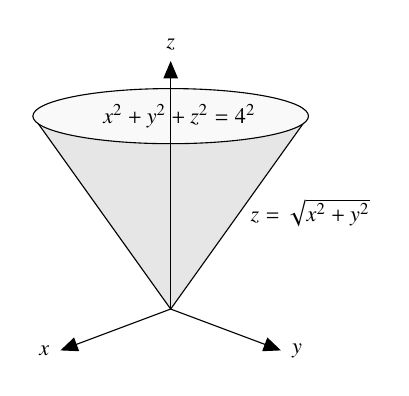
\begin{tikzpicture}[scale=0.7]
      \fill[gray, opacity=0.2]
      (0,0) -- (-2.5,3.5) -- (2.5,3.5) -- (0,0);

      \draw (0,0) -- (-2.5,3.5);  
      \draw (2.5,3.5) -- (0,0) node[midway, right]{$z=\sqrt{x^2+y^2}$};

      \draw[fill=gray!5] (0,3.5) ellipse (2.5 and 0.5);
      \draw[-triangle 45](0,0) -- (2,-0.75) node[right]{$y$};
      \draw[-triangle 45](0,0) -- (-2,-0.75) node[left]{$x$};
      \draw[-triangle 45](0,0) -- (0,4.5) node[above]{$z$};

      \node at (0,3.5) {\ \ \ $x^2+y^2+z^2=4^2$};
   \end{tikzpicture}
   \end{adjustbox}
\end{tabularx}

\vspace{4ex}
\textbf{\mred{Exr.}} Use spherical coordinates to evaluate
$\int_{-2}^2 \int_{-\sqrt{4-x^2}}^{\sqrt{4-x^2}} \int_0^{\sqrt{4-x^2-y^2}} z^2 \sqrt{x^2+y^2+z^2} \,dV$

\Heading{Solution:}

\vspace{-\baselineskip}
\begin{tabularx}{\textwidth}{p{3cm}|p{3cm}|X|p{3cm}}
   $\begin{aligned}
      & x^2+y^2=4 \\
      & \therefore r=2 \\
   \end{aligned}$
   &
   $\begin{aligned}
      & x=r \sin \theta \cos \phi \\
      & y=r \sin \theta \sin \phi \\
      & z=r \cos \theta
   \end{aligned}$
   &
   $\begin{aligned}
      & x^2+y^2+z^2\\
      & = r^2\sin^2\theta\cos^2\phi+r^2\sin^2\theta\sin^2\phi+r^2\cos^2\theta\\
      & = r^2\sin^2\theta\cdot 1+r^2\cos^2\theta\\
      & = r^2
   \end{aligned}$
   &
   $\begin{aligned}
      &\text{Since, \ } z = 0\\
      & \Rightarrow r\cos\theta = 0\\
      & \Rightarrow \cos\theta = \cos\frac{\pi}{2}\\
      & \therefore \theta = \frac{\pi}{2}\\
   \end{aligned}$
\end{tabularx}


\begin{minipage}[t]{0.66\linewidth}
\noindent
   \begin{adjustbox}{valign=t}
      $\begin{aligned}
         & \text{Now, }\\[1ex]
         & \int_{\phi=0}^{2 \pi} \int_{\theta=0}^{\frac{\pi}{2}} \int_{r=0}^2(r\cos\theta)^2 \sqrt{r^2} \ r^2\sin\theta \ \dr\dtheta\dphi\\[1ex]
         & =\int_{\phi=0}^{2 \pi} \dphi \quad
         \int_{r=0}^2 r^5 \dr \quad
         \int_{\theta=0}^{\frac{\pi}{2}}\cos^2\theta\sin\theta\dtheta \\[1ex]
         & =\int_{\phi=0}^{2 \pi} \dphi \quad
         \int_{r=0}^2 r^5 \dr \quad
         \int_1^0 z^2(-dz) \\[1ex]
         & = \left[\Phi\right]_0^{2 \pi} \tab \cdot 
         \left[\frac{r^6}{6}\right]_0^2 \tab \cdot
         \left[-\frac{z^3}{3}\right]_1^0\\[1ex]
         & = 2\pi \cdot \frac{64}{6} \cdot
         \frac{1}{3} \tabs =\frac{64\pi}{9}
      \end{aligned}$
   \end{adjustbox}
\end{minipage}
\begin{minipage}[t]{0.32\linewidth}
\noindent
   \begin{adjustbox}{valign=t}
      \divideX
      $\begin{aligned}
         & \text {Let } \\
         & \cos \theta = z \\
         & \Rightarrow -\sin\theta \dtheta= dz \\
         & \therefore \sin\theta \dtheta= -dz \\[2ex]
         & \text {when } \theta \rightarrow 0 \text { \ to \ } \frac{\pi} {2} \\
         & \text {then } z \rightarrow 1 \text { \ to \ } 0
      \end{aligned}$
   \end{adjustbox}
\end{minipage}




\vspace{4ex}
\textbf{\mred{Exr.}} Use spherical coordinates to evaluate
$\int_{-3}^3 \int_{-\sqrt{9-x^2}}^{\sqrt{9-x^2}} \int_{-\sqrt{9-x^2-y^2}}^{\sqrt{9-x^2-y^2}} \sqrt{x^2+y^2+z^2} \dz\dy\dx$

\Heading{Solution:}
\vspace{-\baselineskip}
\begin{tabularx}{\textwidth}{p{2.5cm}|p{3cm}|X|p{4.2cm}}
   $\begin{aligned}
      & x^2+y^2=9 \\
      & \therefore r=3 \\
   \end{aligned}$
   &
   $\begin{aligned}
      & x=r \sin \theta \cos \phi \\
      & y=r \sin \theta \sin \phi \\
      & z=r \cos \theta
   \end{aligned}$
   &
   $\begin{aligned}
      & x^2+y^2+z^2\\
      & = r^2\sin^2\theta\cos^2\phi+r^2\sin^2\theta\sin^2\phi+r^2\cos^2\theta\\
      & = r^2\sin^2\theta\cdot 1+r^2\cos^2\theta\\
      & = r^2
   \end{aligned}$
   &
   $\begin{aligned}
      &\text{Since, \ } z = 0\\
      & \Rightarrow r\cos\theta = 0\\
      & \Rightarrow \cos\theta = \cos\frac{\pi}{2}\\
      & \therefore \theta = \frac{\pi}{2}\\
      & \text{For whole sphere, } \theta=\pi
   \end{aligned}$
\end{tabularx}

$\begin{aligned}
& \text {Now, }\\[1ex]
& =\int_{\phi=0}^{2 \pi} \int_{\theta=0}^\pi \int_{r=0}^3 \sqrt{r^2} \ r^{2}\sin\theta \dr\dtheta\dphi \\[1ex]
& =\int_{\phi=0}^{2 \pi} \dphi 
\int_{\theta=0}^\pi \sin \theta \dtheta
\int_{r=0}^3 r^3 \dr 
\quad =\left[\phi\right]_0^{2 \pi} \tab
\left[-\cos \theta\right]_0^\pi \tab
\left[\frac{r^4}{4}\right]_0^3 \\[1ex]
& =2 \pi \cdot(-\cos \pi+\cos 0) \cdot \frac{3^4}{4}
\quad =2 \pi \cdot(1+1) \cdot \frac{81}{4} \tabs =81 \pi
\end{aligned}$

% \begin{tikzpicture}
%    \begin{axis}[
%       % hide axis,
%       colormap/viridis,
%       view={135}{10}]
%       \addplot3[surf, shader=interp, opacity=0.5, samples=20, domain=0:360, y domain=0:4, fill=red] (
%          {y*cos(x)},
%          {y*sin(x)},
%          {y});

%       % Axis
%       \addplot3[mark=none, color=black] coordinates {(0,0,0) (1.5,0,0)};
%       \addplot3[mark=none, color=black] coordinates {(0,0,0) (0,1.5,0)};
%       \addplot3[mark=none, color=black] coordinates {(0,0,0) (0,0,5)};

%       \node at (1.75,0,0) {$x$};
%       \node at (0,1.65,0) {$y$};
%       \node at (0,-2,5.5) {$z$};
%     \end{axis}
% \end{tikzpicture}
   
\pagebreak

\CHeading{\cyan{Extremum Principle}}
Let $f(x, y)$ and $g(x, y)$ be two function of two variables $x$ and $y$ with continuous partial derivative on some open set containing the constraint curve $g(x, y)=0$ and assuming that $\vec{\nabla}g(x, y) \neq 0$ at any point on the curve. 
If $f(x,y)$ has a relative extremum at a point $(x_o, y_o)$ on the constraint curve $g(x, y)$ where the gradient vectors $\vec{\nabla} f\left(x_o, y_o\right)$ and $\vec{\nabla} g\left(x_o, y_o\right)$ this are parallel. That is, $\vec{\nabla} f=\lambda \vec{\nabla} g$, for some sealer $\lambda$. This $\lambda$ is called the \textbf{Lagrange} multiplies.

\CHeading{\cyan{Green's Theorem:}}
Let $C$ be a simple closed curve in the $xy$ plane such that a line parallel to either axis cuts $C$ in at most two points.
Let $M(x,y)$, $N(x,y)$, $\frac{\partial N}{\partial x}$, $\frac{\partial M}{\partial y}$ be continuous function of $x$ and $y$ inside and on $C$ and $R$ be the region inside $C$ then, $$\osint[c] M(x,y)\dx+N(x,y)\dy = \miint_S \left(\frac{\partial N}{\partial x} - \frac{\partial M}{\partial y}\right) \dx\dy$$


\CHeading{\cyan{Gauss Theorem}}
The surface integral of the normal component of a continuous diffentiable vector $\vec{F}$ taken over a closed surface $S$ is equal to the integral of the divergence of $\vec{F}$ taken over the volume $V$ enclosed by the surface.

\vspace{-\baselineskip}
\begin{center}
   $\text { Mathematically } \miint_S \left(\vec{F} \cdot \vec{n}\right) \dS =\miiint_V \left(\nabla \cdot \vec{F}\right) \,dV$\\[1.5ex]
   where $n$ is the positive normal to $s$.
\end{center}

\CHeading{\cyan{Stoke's theorem}}
If the components of a vector field $\vec{F}(x,y,z) = f(x,y,z)\vec{i}+g(x,y,z)\vec{j}+h(x,y,z)\vec{k}$ are continuous and have continuous first partial derivatives on some open set $S$ and $C$ be smooth closed curve then, $$\osint[C]\vec{F} \cdot \dvr = \miint_S(\nabla\times\F) \cdot \vec{n} \dS$$
relationship between line and surface integrals a generalization of Green's theorem to three dimensions is called Stoke's theorem.


\CHeading{\cyan{Coordinate System}}
\begin{tabularx}{\textwidth}{p{5cm}|X}
   \begin{tabular}{ll}
      Cartesian &: $(x,y)$ \\
      Polar &: $(r,\theta)$ \\
      Rectangular &: $(x,y,z)$ \\
      Cylindrical &: $(\rho,\phi,z)$ \\
      Spherical &: $(r,\theta,\phi)$ \\
   \end{tabular}
   &
   $\begin{array}{l|l|l}
      \text{Cartesian -- Polar} &
      \text{Rectangular -- Cylindrical} &
      \text{Rectangular -- Spherical}\\
      x=r\cos\theta & x=\rho\cos\phi & x=r\sin\theta\cos\phi\\
      y=r\sin\theta & y=\rho\sin\phi & y=r\sin\theta\sin\phi\\
      & z=z & z=r\cos\theta\\
      |J| = r \dr\dtheta & |J| = \rho\ \drho\dphi\dz & |J| = r^{2}\sin\theta \dr\dtheta\dphi
   \end{array}$
\end{tabularx}
\end{document}